En esta secci\'on se presentan algunos \'arboles de derivaci\'on de cadenas v\'alidas para la gram\'atica presentada.\\

\subsection{Ejemplo 1 - Aritm\'etico}
El siguiente ej\'emplo corresponde a la cadena:\\
$+N / (N-N*N*-N)$
Lo interesante de esta cadena es ver que no genera ambiguedades con el uso de los signos para los n\'umeros.
%~ \begin{figure}[!h]
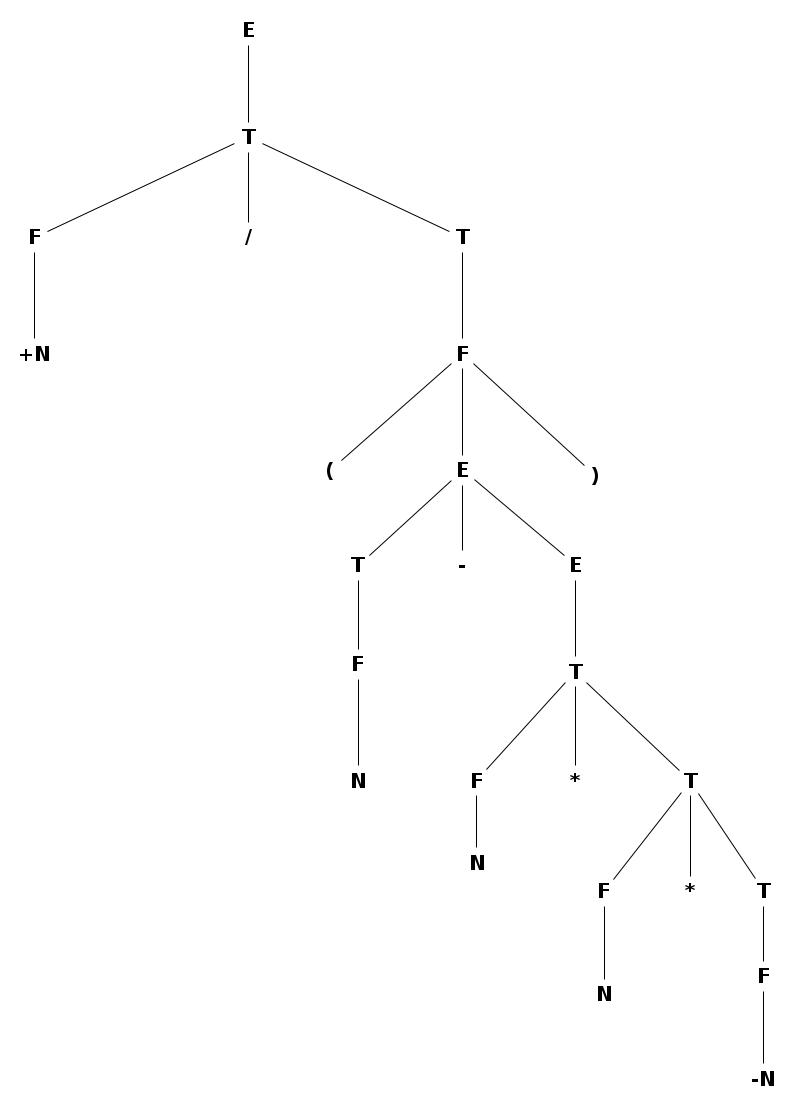
\includegraphics[scale=0.40]{arboles_derivacion/ejemplo1.jpg}
%~ \end{figure}
\subsection{Ejemplo 2 - Aritm\'etico}
El ej\'emplo 2 se corresponde a la cadena:
$N*N+N*N$
%~ \centerline{
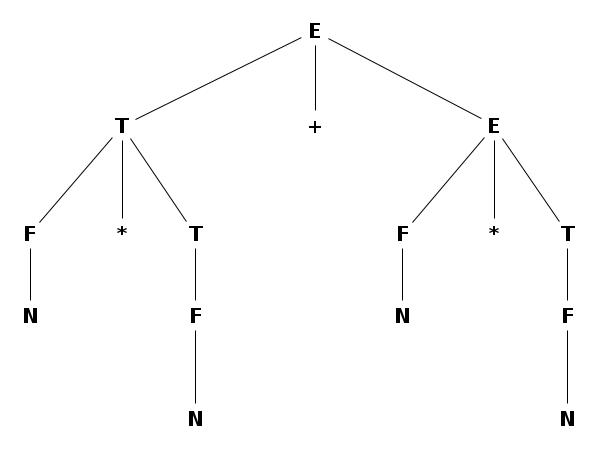
\includegraphics[scale=0.40]{arboles_derivacion/ejemplo2.jpg}
%~ }


\subsection{Ejemplo 3 - Programa v\'alido}
El siguiente \'arbol de derivaci\'on se corresponde con la siguiente expresi\'on.

\lstinputlisting[language=Python,breaklines=true]{../Ejemplos/eg22.peg}

Por motivos de mejor visualizaci\'on se decidi\'o partir en partes este \'arbol. Las partes consisten en El comienzo del mismo, que se divide en 2 ramas, y luego cada una se van a presentar a continuaci\'on.
\\
Para una mejor comprensi\'on de los cortes se muestran los mismos con asterisco y un n\'umero.

\centerline{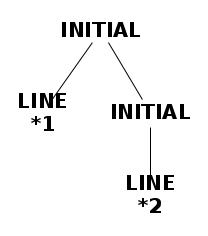
\includegraphics[scale=0.40]{arboles_derivacion/union_cube1_cube2.jpg}}

\centerline{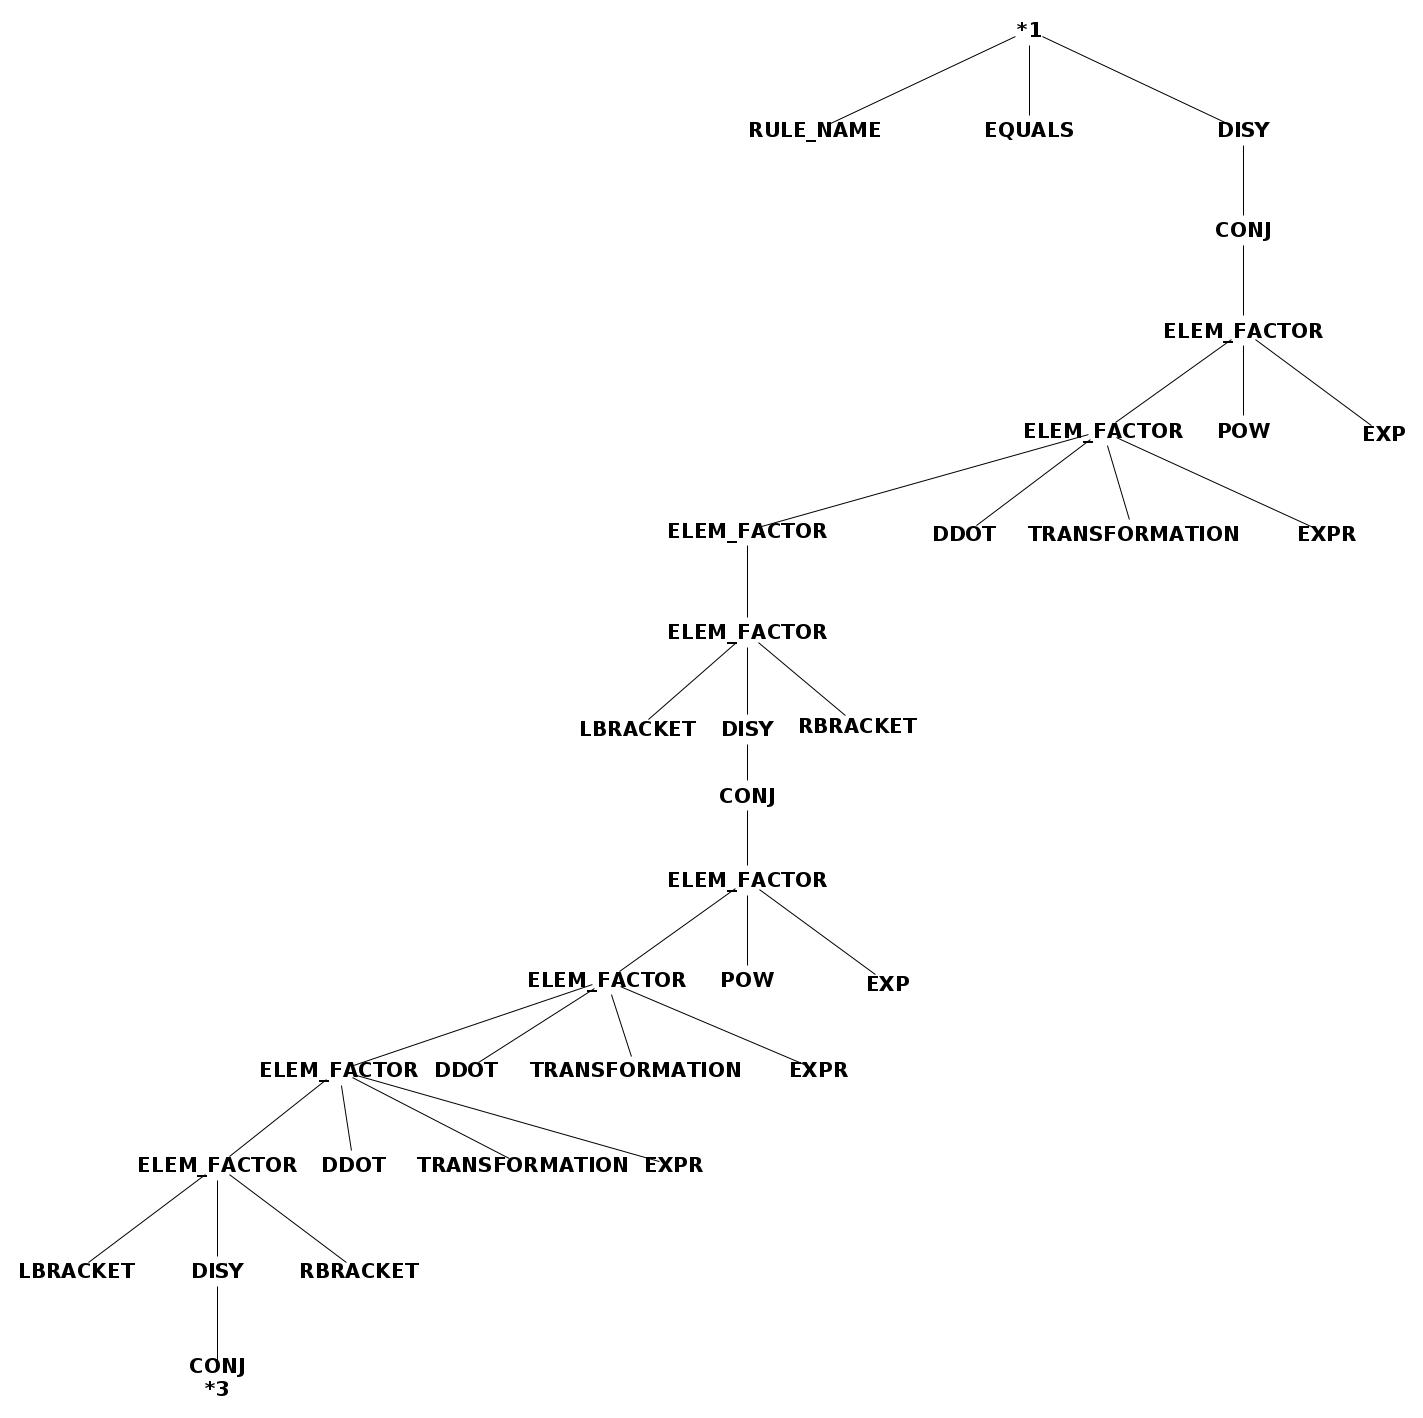
\includegraphics[scale=0.40]{arboles_derivacion/cube1.jpg}}

\centerline{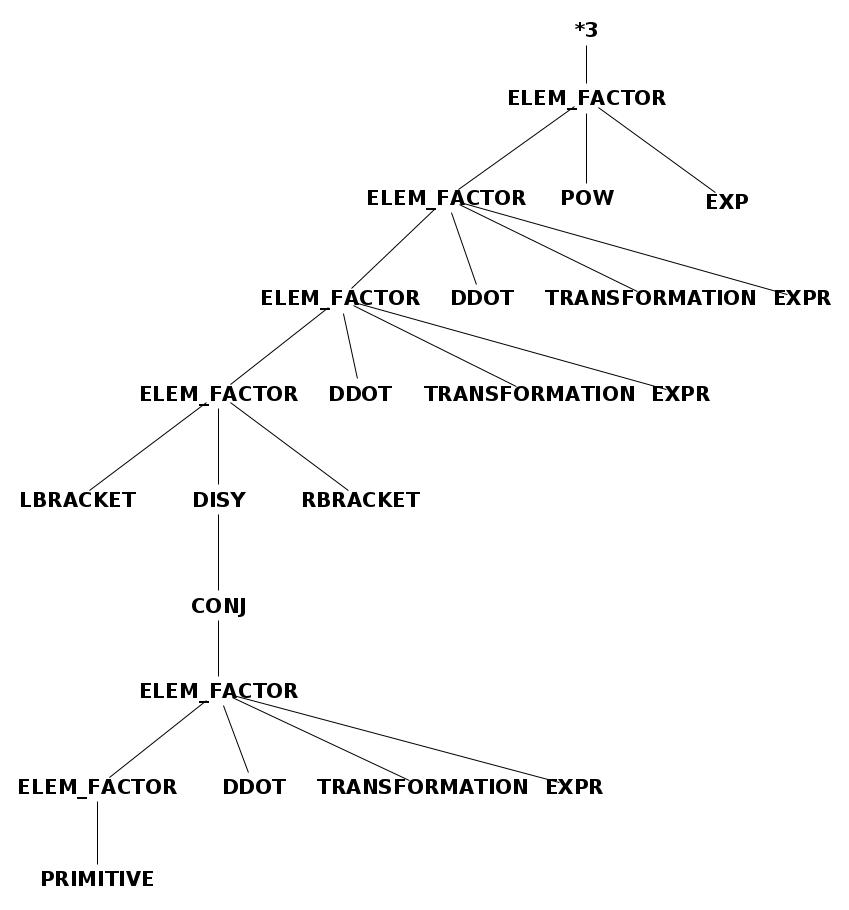
\includegraphics[scale=0.40]{arboles_derivacion/cube1b.jpg}}

\centerline{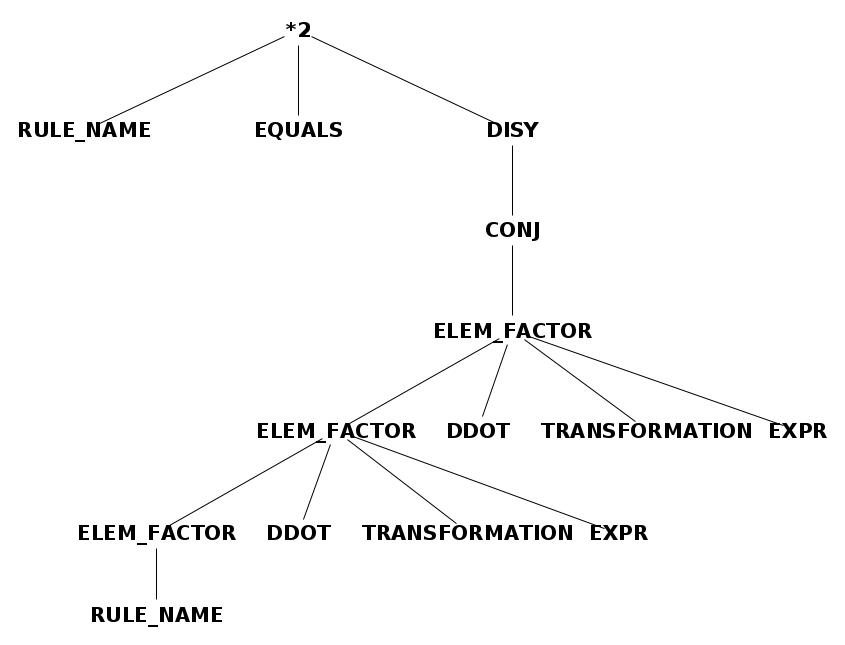
\includegraphics[scale=0.40]{arboles_derivacion/cube2.jpg}}



\subsection{Ejemplo 4 - Programa v\'alido}
El siguiente ejemplo muestra el \'arbol de derivaci\'on para la siguiente expresi\'on.

\lstinputlisting[language=Python,breaklines=true]{../Ejemplos/eg09.peg}

\centerline{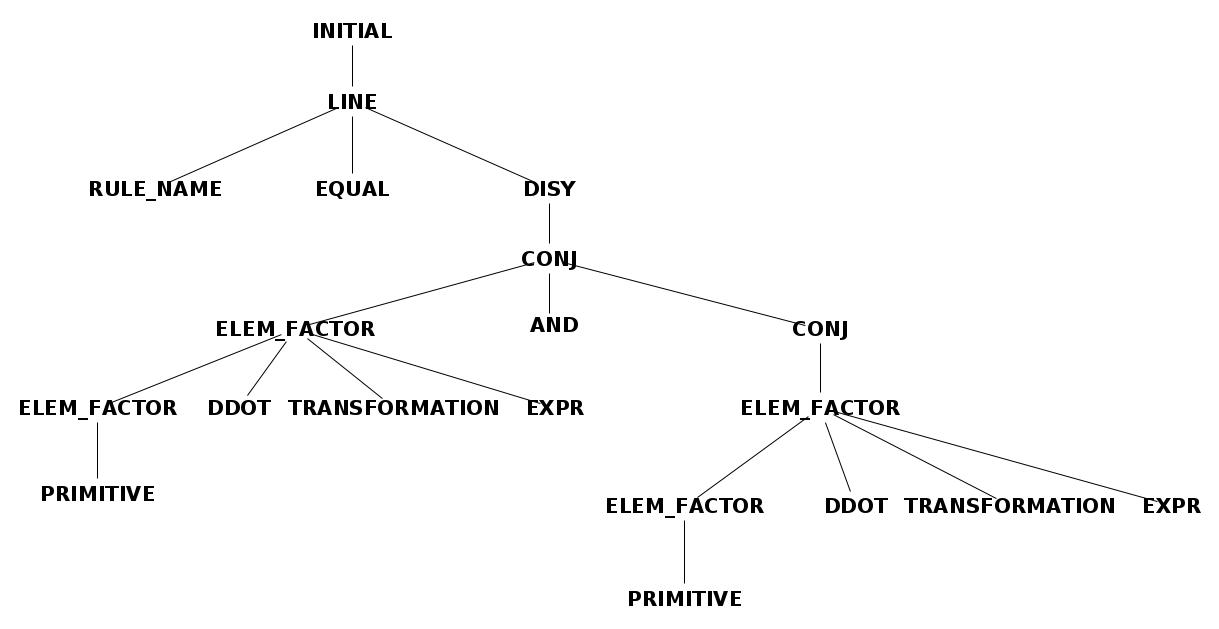
\includegraphics[scale=0.40]{arboles_derivacion/Ejemplo_and1.jpg}}

\subsection{Ejemplo 5 - Programa v\'alido}

El siguiente ejemplo muestra el \'arbol de derivaci\'on para la siguiente expresi\'on.

%\lstinputlisting[language=Python,breaklines=true]{../Ejemplos/eg09b.peg}

\centerline{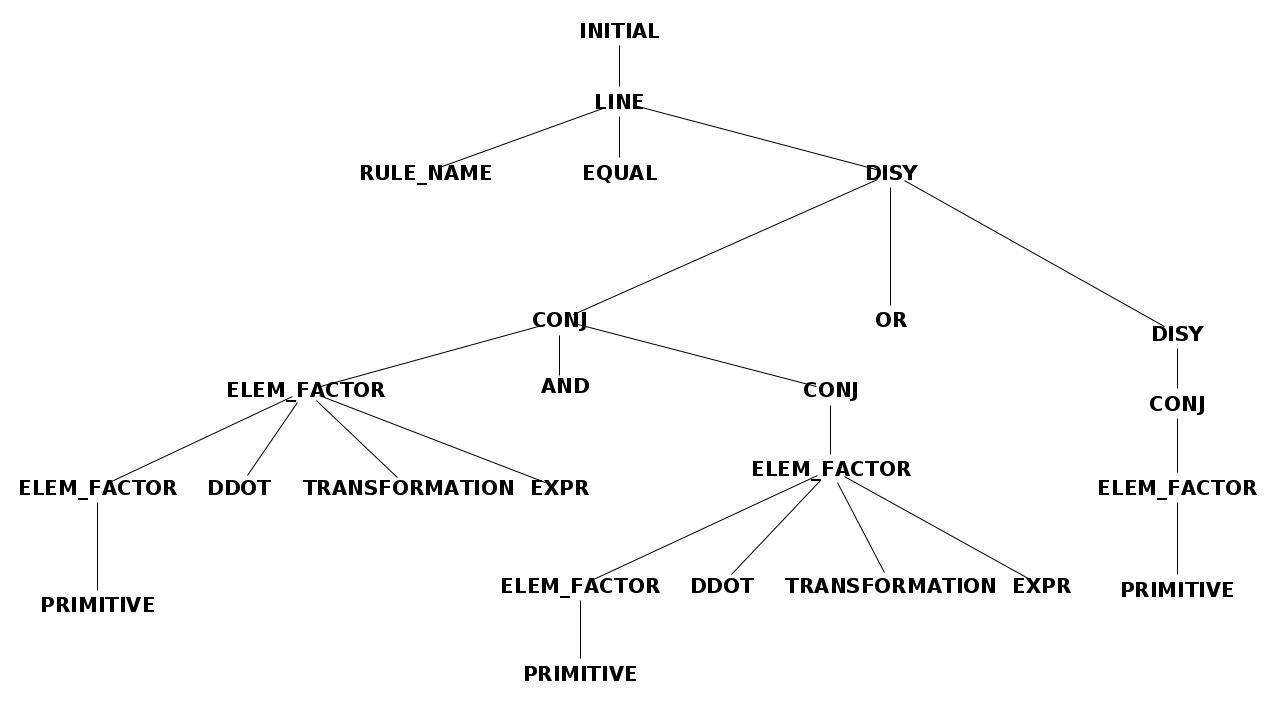
\includegraphics[scale=0.40]{arboles_derivacion/Ejemplo_and_or1.jpg}}

\subsection{Ejemplo 6 - Programa v\'alido}

El siguiente ejemplo muestra el \'arbol de derivaci\'on para la siguiente expresi\'on.

\lstinputlisting[language=Python,breaklines=true]{../Ejemplos/eg14.peg}

\centerline{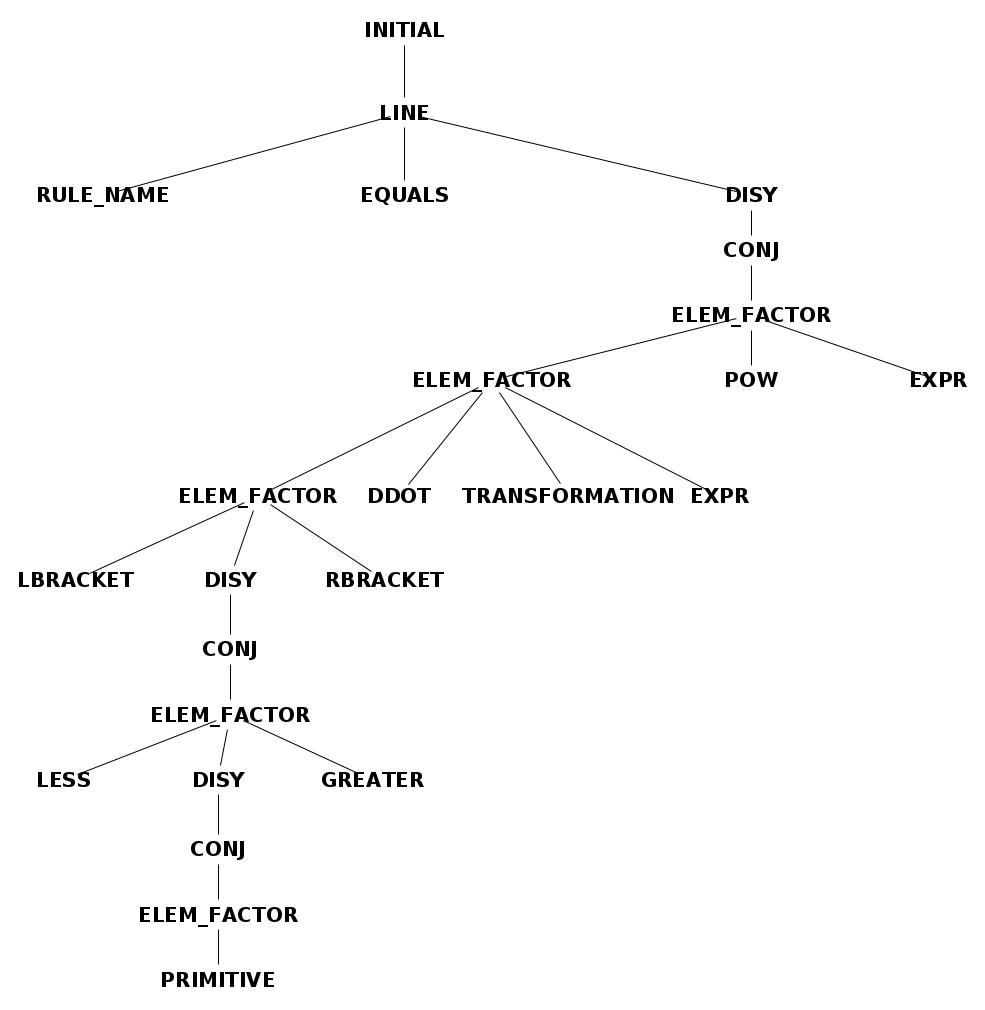
\includegraphics[scale=0.40]{arboles_derivacion/brackets_less_greater1.jpg}}
